% Allow relative paths in included subfiles that are compiled separately
% See https://tex.stackexchange.com/questions/153312/
\providecommand{\main}{..}
\documentclass[\main/thesis.tex]{subfiles}

\begin{document}

\chapter{Background Information}
\chaptermark{background}
\label{chp:background}

In this chapter, I give a brief overview of the anatomy of a human heart.
Next, I describe the characteristics of a standard 12-lead \gls{ecg} and the notable waves in a \gls{ecg} signal.
I then give an overview of the \emph{PhysioNet/CinC 2020 Challenge} task/objective, provided dataset of \gls{ecg} records, and definitions for the diagnoses we are tasked to predict.

\section{Heart Anatomy and Electrical Conduction System}

\begin{figure}[ht]
    \centering
    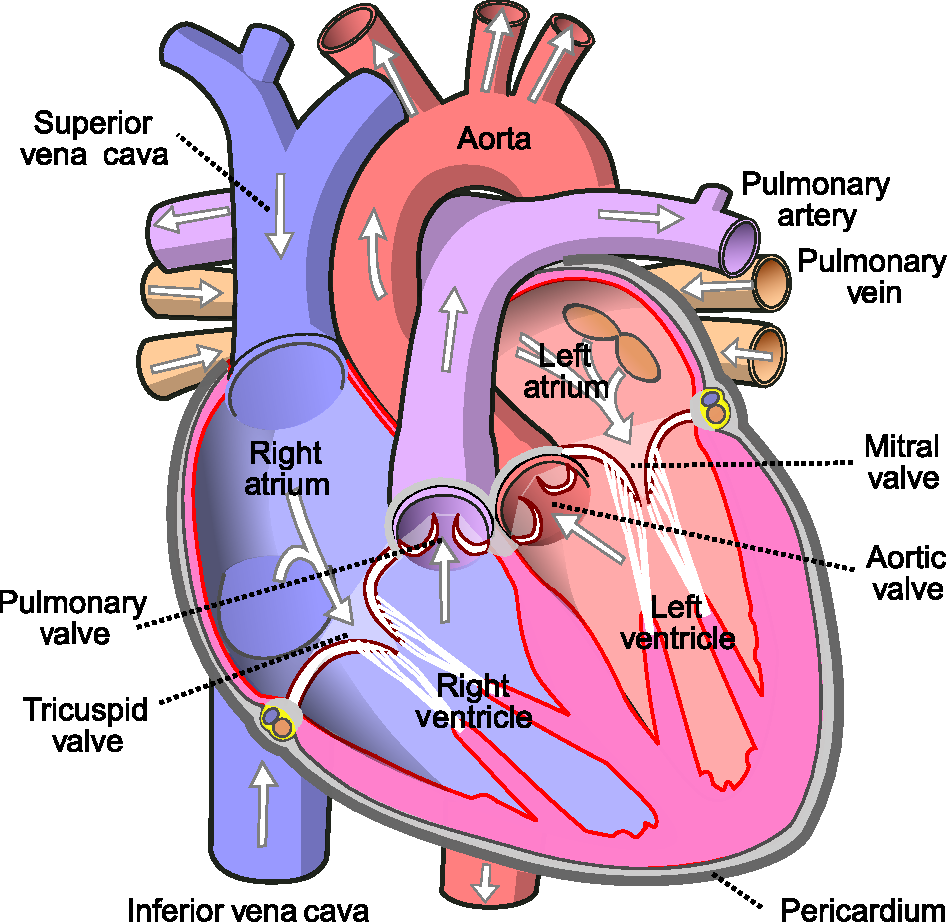
\includegraphics[width=8cm]{figure/Diagram_of_the_human_heart.pdf}
    \caption[Anterior, anatomical view of the structures of a human heart.]{Anterior, anatomical view of a human heart. The primary valves and chambers of the heart are annotated, with arrows indicating the direction of blood flow due to the contractions of the cardiac chambers.
    Image licensed \texttt{CC BY-SA 3.0} from Wikipedia user \href{https://en.wikipedia.org/wiki/User:Wapcaplet}{Wapcaplet}, source: \url{https://en.wikipedia.org/wiki/Heart\#/media/File:Diagram\_of\_the\_human\_heart\_(cropped).svg}
    }
    \label{fig:heart_anatomy}
\end{figure}

A high level overview of the primary valves and chambers within the heart can be found in Figure~\ref{fig:heart_anatomy}.
The upper chambers of the heart, consisting of the right and left atriums, work in cooperation with the lower chambers of the heart, consisting of the left and right ventricles.
The right ventricle pushes blood into the pulmonary artery which connects to the lungs to return oxygenated blood.
The oxygenated blood returns to the heart through the pulmonary veins and enters into the left atrium.
The left atrium collects ad pumps the oxygenated blood into the left ventricle through the mitral valve.
The left ventricle pumps the oxygenated blood out of the heart to the rest of the body through the aorta.
The deoxygenated blood is collected back into the heart through the superior and inferior vena cava and into the right atrium.
The cycle repeats as the right atrium pumps the blood into the right ventricle through the tricuspid valve, allowing the lungs to once again oxygenate the blood.

\begin{figure}[ht]
    \centering
    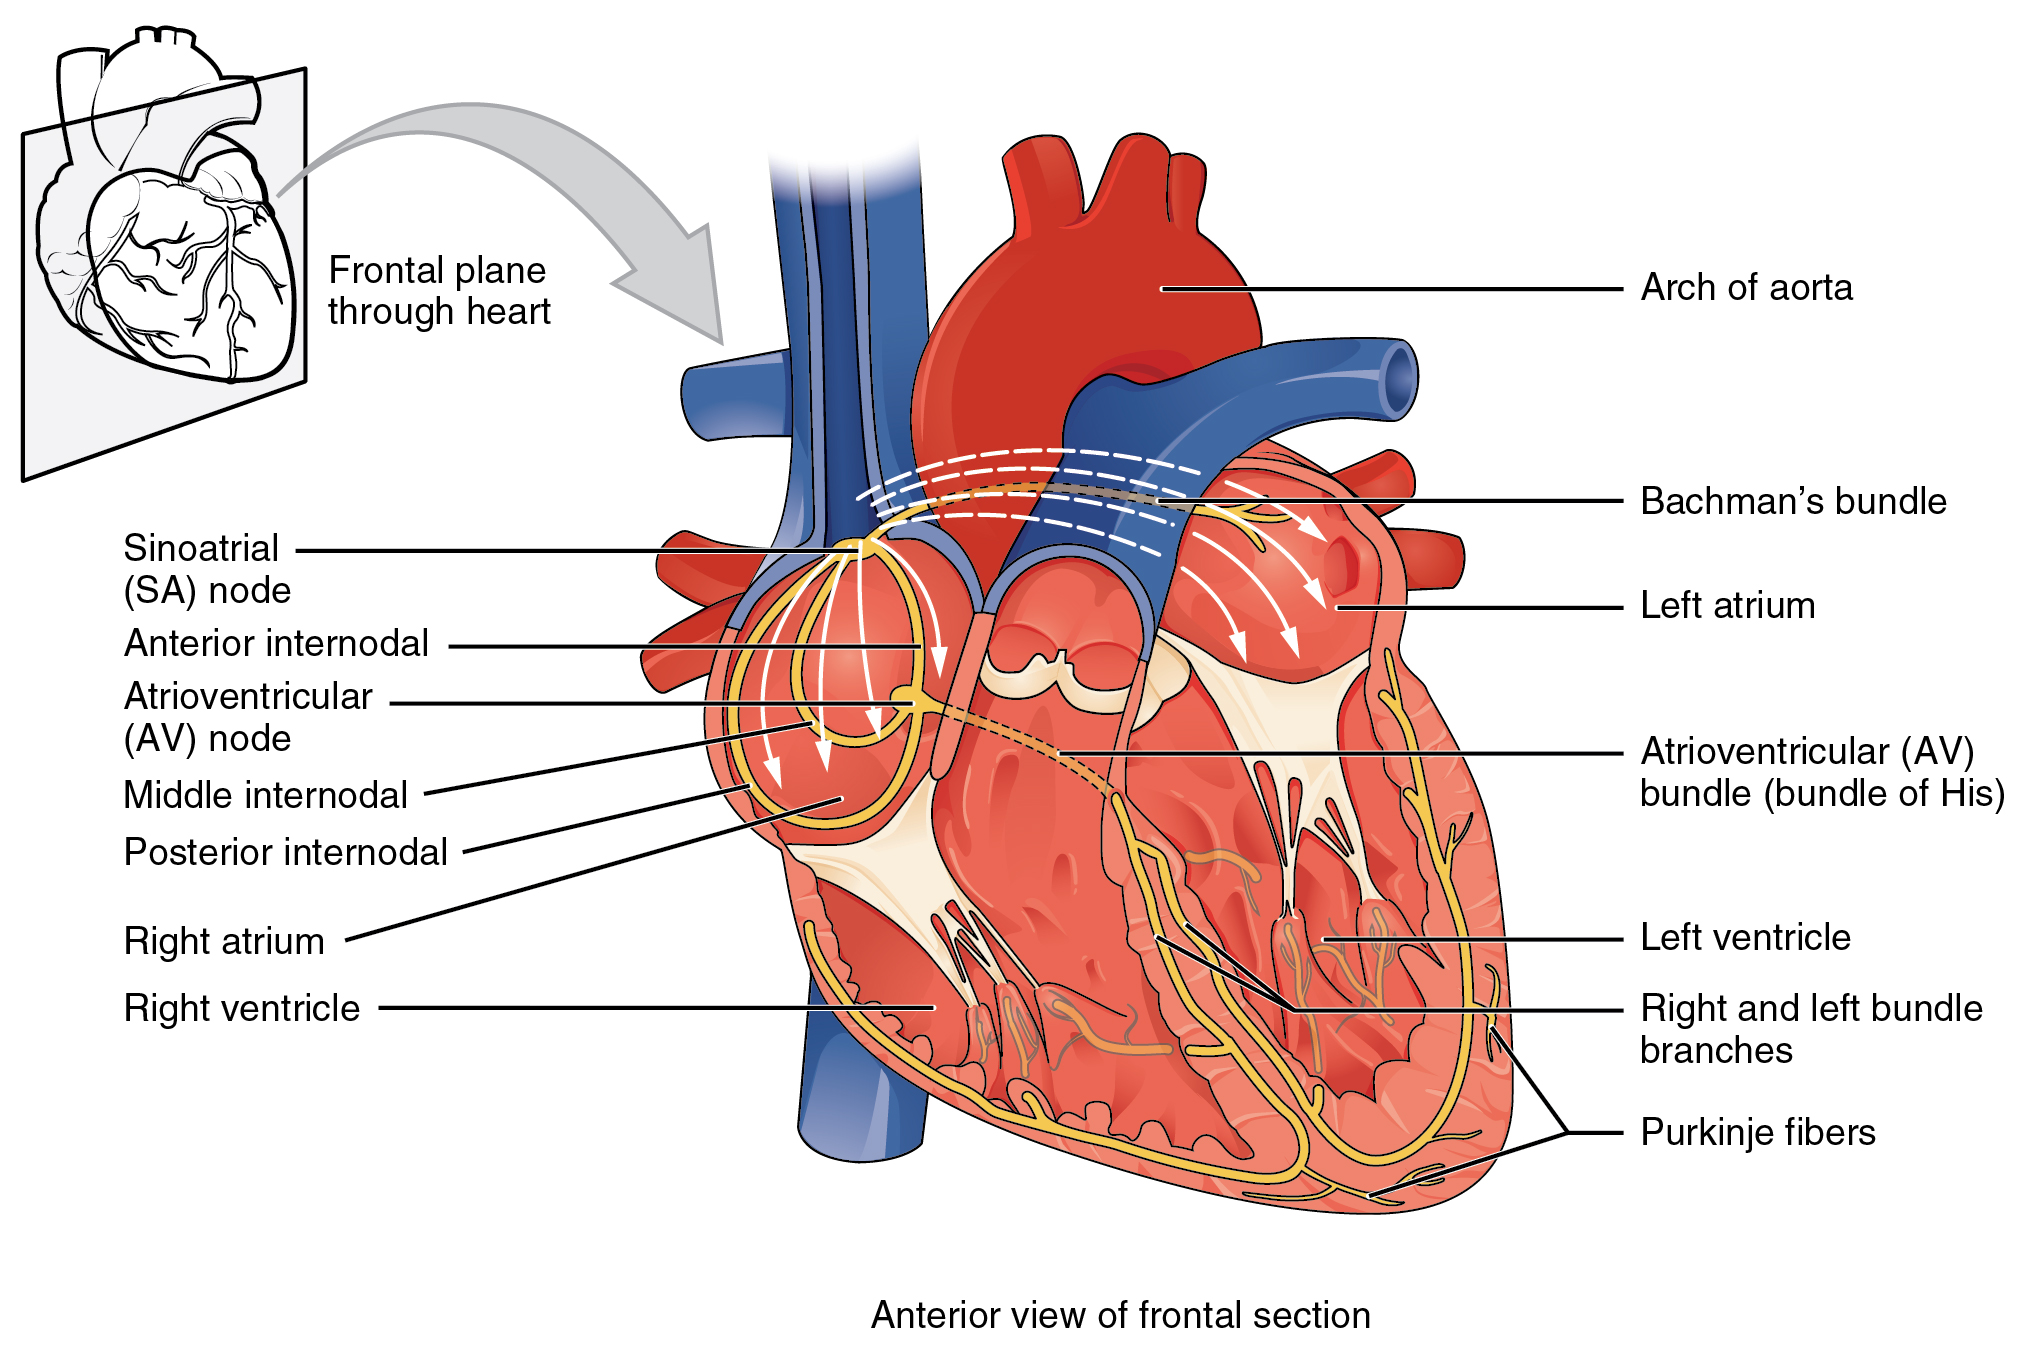
\includegraphics[width=13cm]{figure/conduction-system-of-the-heart.jpeg}
    \caption[Anterior, anatomical view of the conduction system of a human heart.]{Anterior, anatomical view of the conduction system of a human heart. The conducting components of the heart begin with the sinoatrial node and include the internodal pathways, the atrioventricular node, the atrioventricular bundle, the right and left bundle branches, and the Purkinje fibres.
    Image licensed \texttt{CC BY 4.0} from Betts \emph{et al}~\cite{betts-anatomy-and-physiology} on the OpenStax platform, source: \url{https://openstax.org/books/anatomy-and-physiology/pages/19-2-cardiac-muscle-and-electrical-activity\#fig-ch20_02_02}}
    \label{fig:heart_conduction_system}
\end{figure}

Figure~\ref{fig:heart_conduction_system} shows an overview of the primary structures relevant to the cardiac conduction cycle.
Starting at rest, the sinoatrial node initiates an action potential which travels across the right and left atria.
Once the action potential reaches the atrioventricular node, a ~100ms delay occurs to allow the blood to finish pumping by the atria before the impluse is sent to the atrioventricular bundle.
Once the delay finishes, the impluse sweeps across the atrioventricular bundle, right and left bundle branches to the Purkinje fibers.
The impulse ends at the contractile fibers of the ventricle, at which ventricular contraction begins.

\begin{figure}[ht]
    \centering
    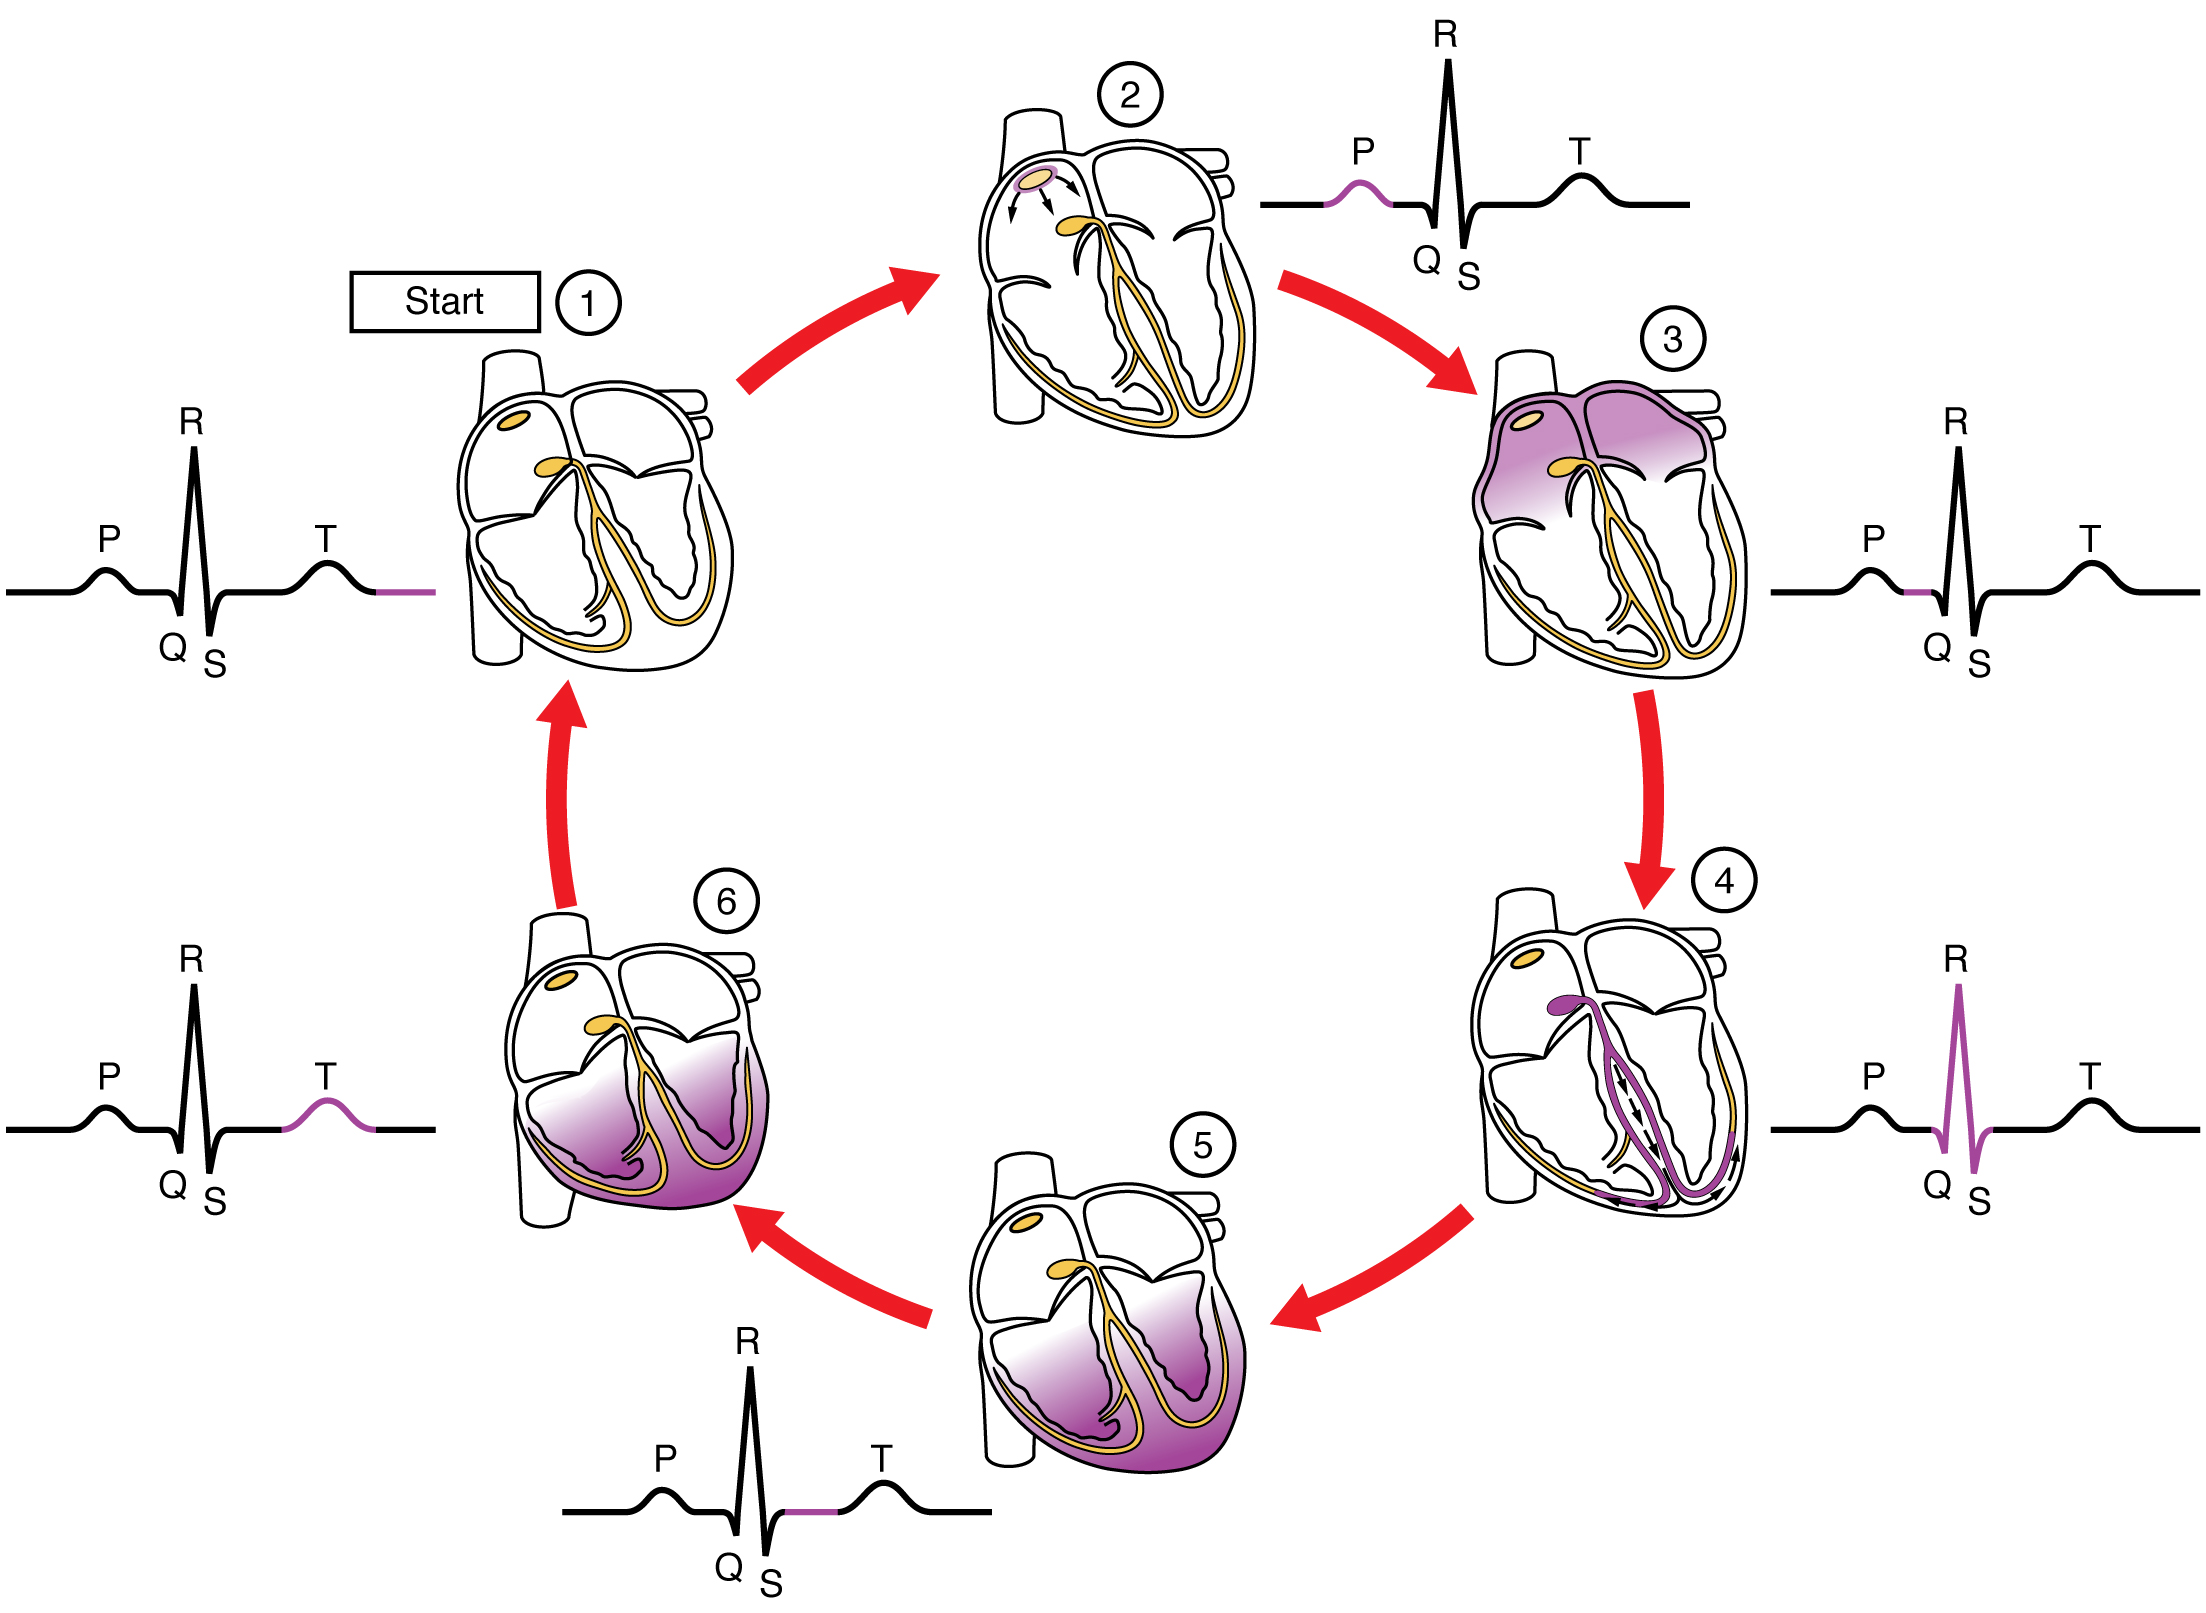
\includegraphics[width=13cm]{figure/pqrst_with_heart_conduction_system.jpeg}
    \caption[Cardiac conduction correlated to ECG tracing waves.]{Cardiac conduction correlated to ECG tracing waves.
    1. The conduction system of the heart is currently at rest, with the ventricles repolarized.
    2. The sinoatrial node begins an action potential which permeates across the atria, causing the \gls{ecg} P wave formation.
    3. A 100ms delay in the impulse occurs which allows the atria to complete pumping blood, showing as the PR segment in the \gls{ecg}.
    4. The impulse proceeds through the atrioventricular bundle and bundle branches to the Purkinje fibers, appearing as the QRS complex in the \gls{ecg}.
    5. The contractile fibers of the ventricles are stimulated by the impulse, causing the ventricles to contract and appears as the ST-segment in the \gls{ecg}.
    6. The impulse dissipates and the ventricular muscles relax, causing the \gls{ecg} T wave formation.
    Image licensed \texttt{CC BY 4.0} from Betts \emph{et al}~\cite{betts-anatomy-and-physiology} on the OpenStax platform, source: \url{https://openstax.org/books/anatomy-and-physiology/pages/19-2-cardiac-muscle-and-electrical-activity\#fig-ch20_02_08}}
\end{figure}

\section{Electrocardiogram Tracing}

\begin{figure}[ht]
    \centering
    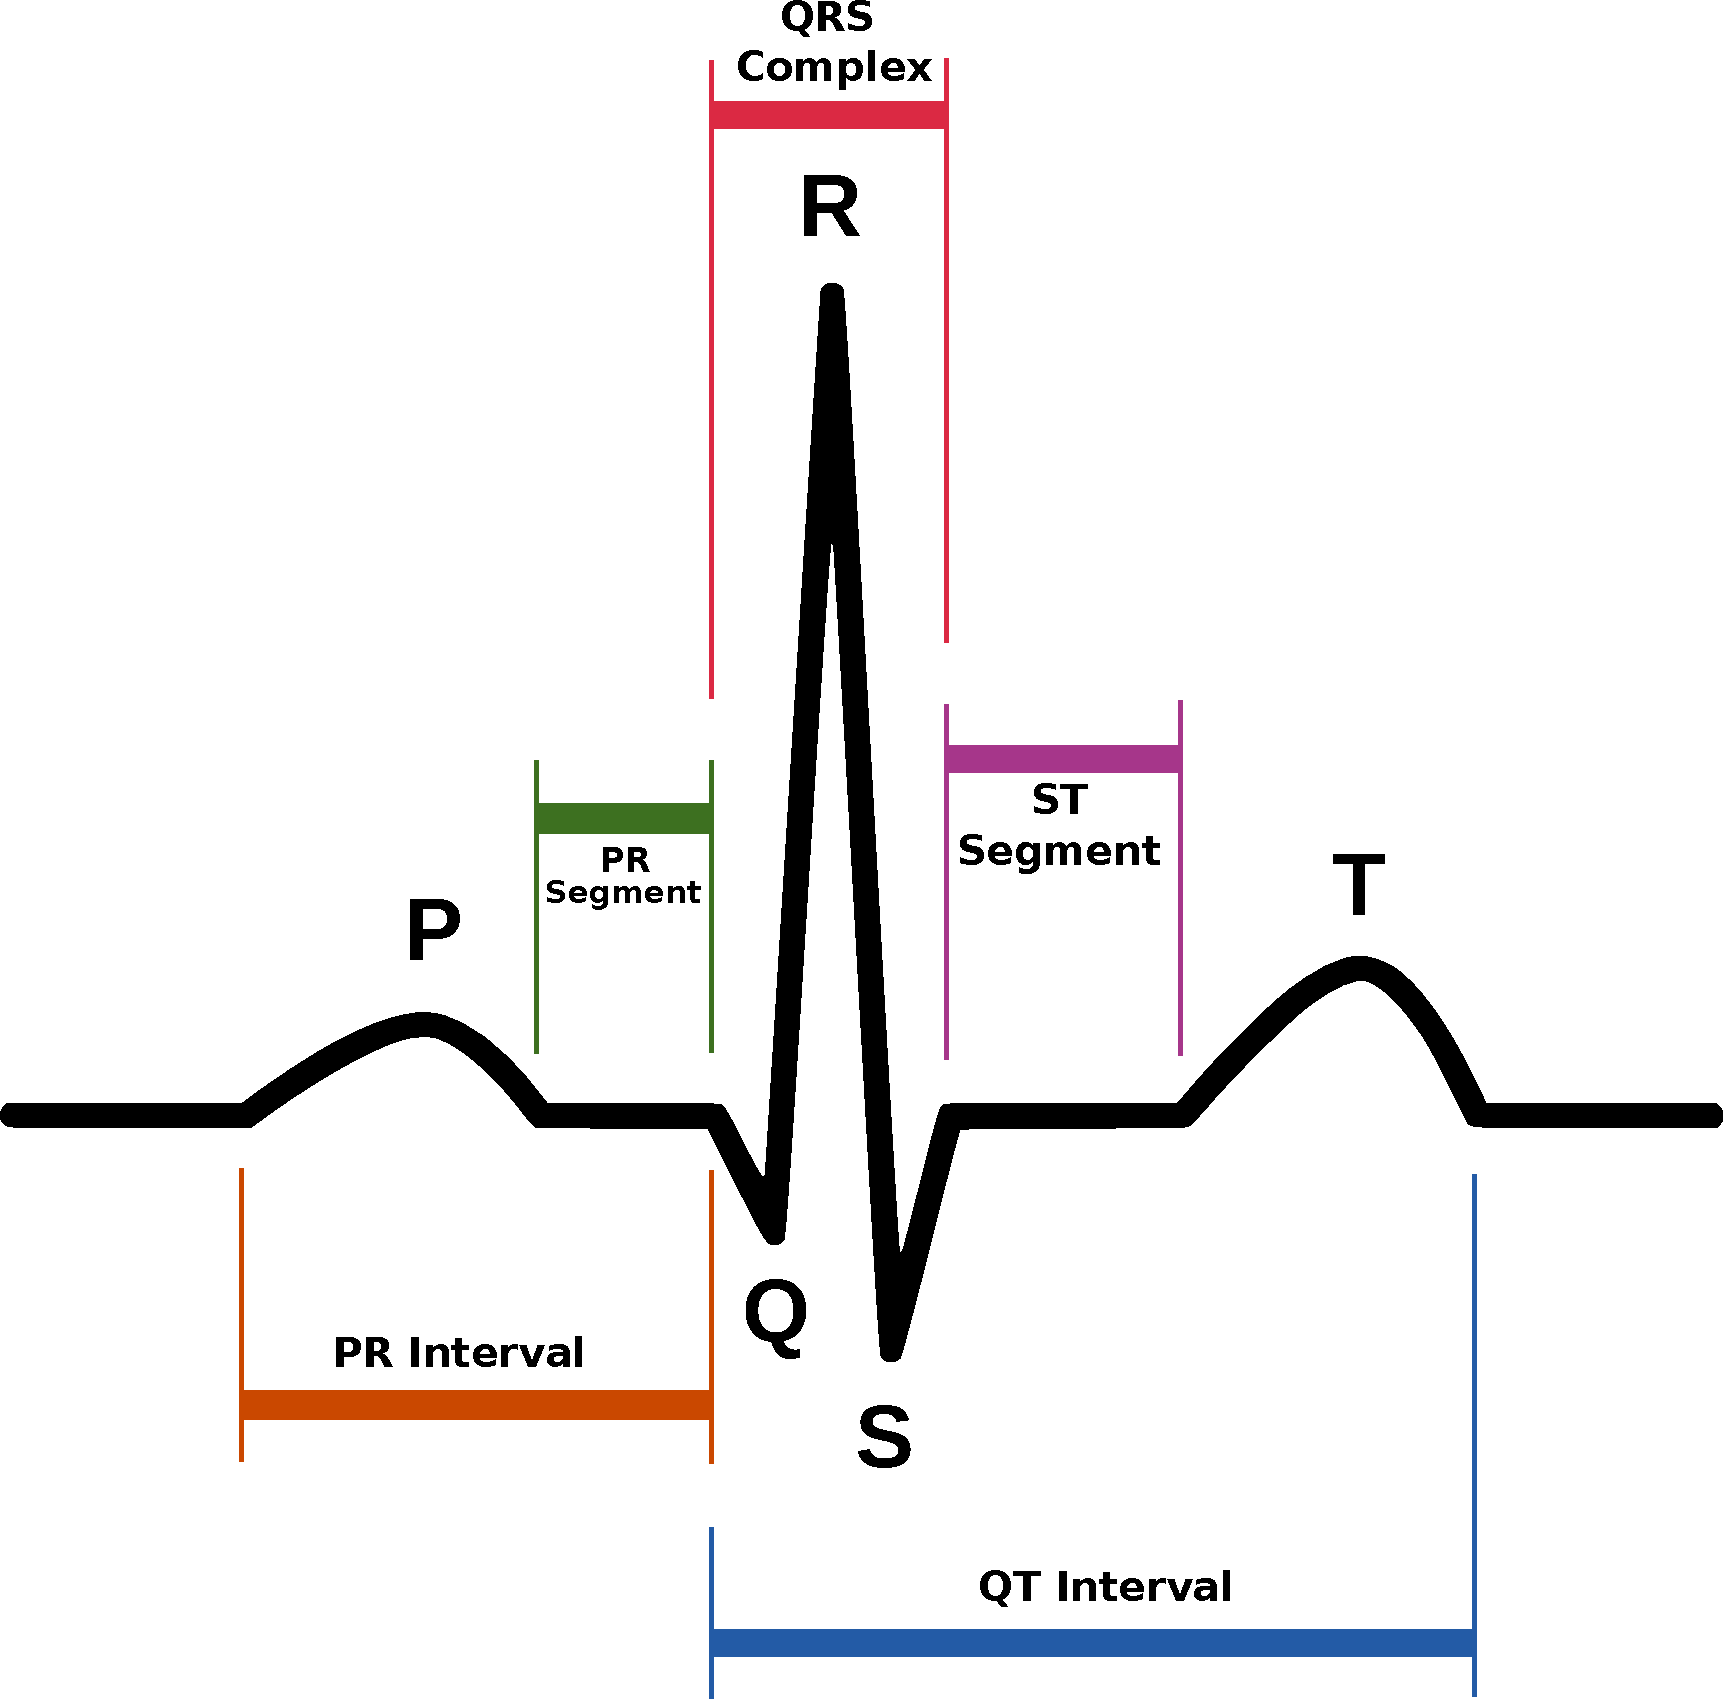
\includegraphics[width=8cm]{figure/PQRST_NormalSinusRhythm.pdf}
    \caption[Normal sinus rhythm \gls{ecg} tracing with PQRST peaks annotated.]{Normal sinus rhythm \gls{ecg} tracing showing the PQRST peaks, the P wave, QRS complex, and T wave along with the PR and QT intervals, plus the PR and ST segments.
    Image belonging to \texttt{public domain} attributed to Anthony Atkielski, source: \url{https://en.wikipedia.org/wiki/Electrocardiography\#/media/File:SinusRhythmLabels.svg}
    }
    \label{fig:pqrst_nsr}
\end{figure}

Within a typical \gls{ecg}, there are five major peaks which make up three major components of the wave as shown in Figure~\ref{fig:pqrst_nsr}.
The P wave captures the depolarization of the atria and represents the contraction of the atria.
The QRS complex captures the depolzarization of the ventricles and represents the contraction of the ventricles.
The T wave captures the repolarization of the ventricles and represents the relaxation of the ventricles.


\section{Predicted Diagnoses}

\begin{description}
    \item[\gls{iavb}] TODO: Describe IAVB.
\end{description}

\gls{af}
\gls{afl}
\gls{brady}
\gls{crbbb}
\gls{irbbb}
\gls{lanfb}
\gls{lad}
\gls{lbbb}
\gls{lqrsv}
\gls{nsivcb}
\gls{pr}
\gls{pac}
\gls{pvc}
\gls{lpr}
\gls{lqt}
\gls{qab}
\gls{rad}
\gls{rbbb}
\gls{sa}
\gls{sb}
\gls{snr}
\gls{stach}
\gls{svpb}
\gls{tab}
\gls{tinv}
\gls{vpb}

% We plot an equation in figure \ref{fig:plot}.

% \begin{figure}
%     \centering
%     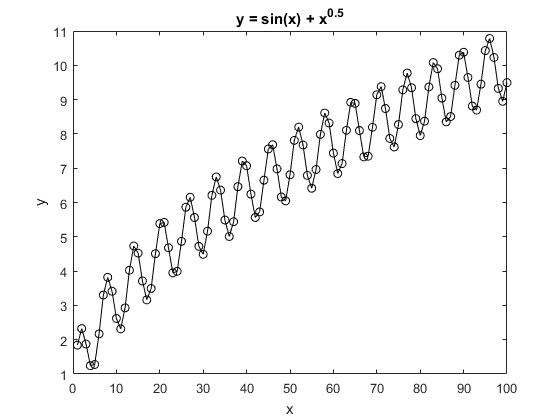
\includegraphics[keepaspectratio=true, width=0.9\textwidth]{\main/figure/plot}
%     \caption[A supporting figure] {A graph of $y = \sin(x) + \sqrt{x}$}
%     \label{fig:plot}
%     % Put the label *after* the caption, but inside the float
% \end{figure}

\end{document}